\documentclass{article} % For LaTeX2e
\usepackage[legalpaper, margin=0.16in]{geometry}
\usepackage{amsmath}
\usepackage{amsfonts,dsfont}
\usepackage{amssymb}
\usepackage[ruled,vlined]{algorithm2e}

\usepackage{graphicx}
\usepackage{caption}
\usepackage{subcaption}
\usepackage{xcolor}
\usepackage{siunitx}

\begin{document}

\begin{figure}
	\centering
	\captionsetup{labelformat=empty}
	\begin{subfigure}[b]{1.0\textwidth}
		%% trim=left bottom right top
		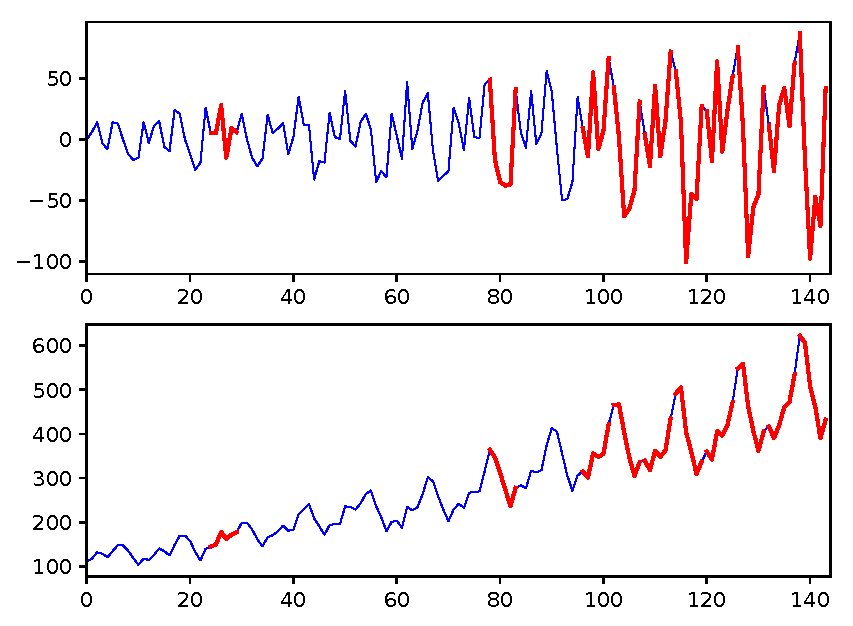
\includegraphics[width=\textwidth, clip=true, trim=0mm 0mm 0mm 0mm]{timeseries_shingles_airline_w6_ifor}
		\label{fig:airline}
	\end{subfigure}
	\caption{Airline dataset: Shingle-based time-series outlier detection. The window size was set to $6$ and the anomaly detector employed was \textit{Isolation Forest}. Since a clear trend is present, we first de-trend the series by differencing with lag $1$. The \textbf{top row} shows the outlier windows detected in the de-trended series. The \textbf{bottom row} shows the corresponding outliers in the original series. In both plots, the outlier windows are shown in \textcolor{red}{red}. \textbf{Note:} There is no separate train or test set in this shingle-based approach.}
	\label{fig:shingles_airline}
\end{figure}

\begin{figure}
	\centering
	\captionsetup{labelformat=empty}
	\begin{subfigure}[b]{1.0\textwidth}
		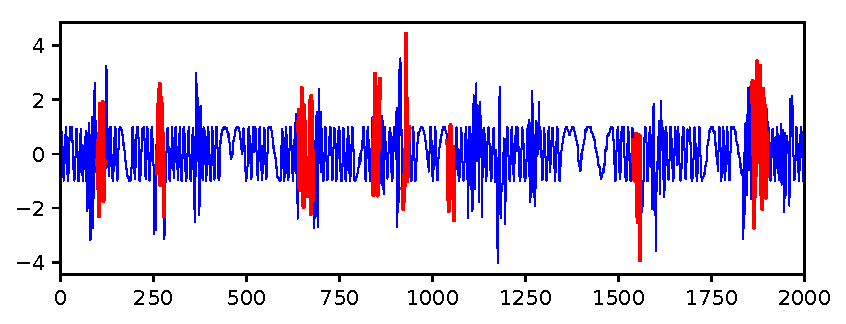
\includegraphics[width=\textwidth, clip=true, trim=0mm 0mm 0mm 0mm]{timeseries_shingles_synthetic_w20_autoenc}
		\label{fig:autoenc}
	\end{subfigure}
    \caption{Synthetic dataset: Shingle-based time-series outlier detection. The window size was set to $20$ and the anomaly detector employed was an \textit{autoencoder}. Since there is no trend in the original data, we did not apply and de-trending operation and the outlier windows are shown in the original timeseries data. The outlier windows are shown in \textcolor{red}{red}. \textbf{Note:} There is no separate train or test set in this shingle-based approach.}
	\label{fig:synthetic}
\end{figure}

\end{document}
